\chapter{运动学牛顿定律习题课}
\section{作业习题}
\subsection*{一、填空题}
\begin{enumerate}
    \item 升降机内地板上放有物体$A$, 其上再放另一物体$B$, 二者的质量分别为$M_A$、$M_B$.当升降机以加速度$a$向下加速运动时$(a<g)$, 物体$A$对升降机地板的压力大小$N=\nl$.  
    \item 如图所示 \ref{fig:12} , 一个小物体$A$靠在一辆小车的竖直前壁上,$A$和车壁间静摩擦系数是$\mu_s$,若要使物体$A$不致掉下来,小车的加速度的最小值应为$a=\nl$.
    \begin{figure}[H]
        \centering
        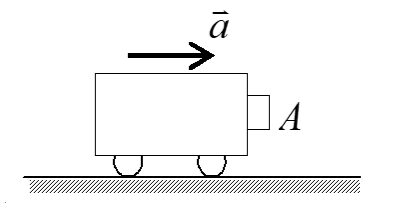
\includegraphics[width=0.15\textheight]{fig12}
            \caption{如图}\label{fig:12}
    \end{figure}
    \item 如图 \ref{fig:13} , 一圆锥摆摆长为$l$、摆锤质量为$m$,在水平面上作匀速圆周运动,摆线与铅直线夹角$\theta$,则摆线的张力$T=\nl$.摆锤的速率$v=\nl$.
    \begin{figure}[H]
        \centering
        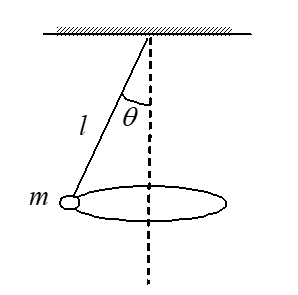
\includegraphics[width=0.15\textheight]{fig13}
            \caption{如图}\label{fig:13}
    \end{figure}
\end{enumerate}
\subsection*{二、选择题}
\begin{enumerate}
    \item  如图 \ref{fig:14} , 一只质量为$m$的猴,原来抓住一根用绳吊在天花板上的质量为$M$的直杆,悬线突然断开,小猴则沿杆子竖直向上爬以保持它离地面的高度不变,此时直杆下落的加速度为(\hspace{1pc})
    \fourch{$g$ ;}{$\frac{m}{M}g$ ;}{$\frac{M+m}{M-m}g$ ;}{$\frac{M+m}{M}G$ .}
    \begin{figure}[ht]
        \centering
        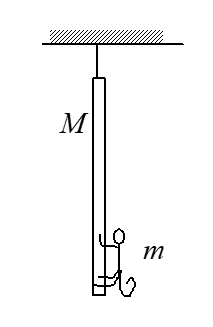
\includegraphics[width=0.06\textheight]{fig14}
            \caption{如图}\label{fig:14}
    \end{figure}
    \item 一段路面水平的公路,转弯处轨道半径为$R$,汽车轮胎与路面间的摩擦系数为$\mu$,要使汽车不致于发生侧向打滑,汽车在该处的行驶速率(\hspace{1pc})
    \twoch{不得小于$\sqrt{\mu gR}$ ;}{不得大于$\sqrt{\mu gR}$ ;}{必须等于$\sqrt{2gR}$ ;}{还应由汽车的质量$M$决定 .}
    \item 质量分别为$m_1$和$m_2$的两滑块$A$和$B$通过一轻弹簧水平连结后置于水平桌面上,滑块与桌面间的摩擦系数均为$\mu$,系统在水平拉力$F$作用下匀速运动,如图所示\ref{fig:15}。如突然撤消拉力,则刚撤消后瞬间,二者的加速度$a_A$和$a_B$分别为(\hspace{1pc}) 
    \begin{figure}[ht]
        \begin{minipage}[ht]{0.4\linewidth}
           \begin{table}[H]
               \begin{tabular}{c}
                  \qquad   (A)\ $a_A=0, a_B=0$;\\
                  \qquad  (B)\ $a_A>0, a_B<0$;\\
                  \qquad  (C)\ $a_A<0, a_B>0$;\\
                  \qquad  (D)\ $a_A<0, a_B=0$.
               \end{tabular}
           \end{table}
        \end{minipage}
        \begin{minipage}[H]{0.5\linewidth}
            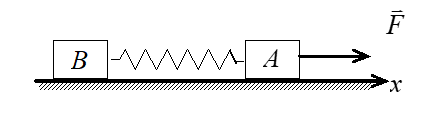
\includegraphics[width=0.25\textheight]{fig15}
            \caption{如图}\label{fig:15}
        \end{minipage}
    \end{figure}
\end{enumerate}
\subsection*{三、计算题}
\begin{enumerate}
    \item 质量为$m$的质点沿$x$轴正向运动: 设质点通过坐标点为$x$时的速度为$v=kx$($k$为常数), 求作用在质点的合外力及质点从$x=x_0$到$x=2x_0$处所需的时间$t$.
    \item 如图 \ref{fig:16}, 在光滑水平桌面上,有两个物体$A$和$B$紧靠在一起.它们的质量分别为$m_A=2kg$, $m_B=1kg$. 今用一水平力$F=3N$推物体$B$,求$B$推$A$的力$f$. 
    \begin{figure}[ht]
        \centering
        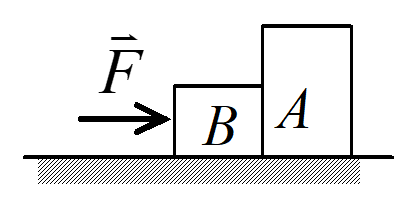
\includegraphics[width=0.15\textheight]{fig16}
            \caption{如图}\label{fig:16}
    \end{figure}
    \item 如图所示 \ref{fig:17}, 质量为$m$的物体用细绳水平拉住,静止在倾角为$\theta$的固定的光滑斜面上,求斜面给物体的支持力.
    \begin{figure}[H]
        \centering
        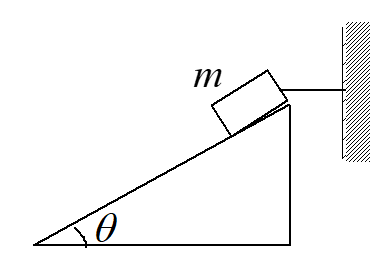
\includegraphics[width=0.15\textheight]{fig17}
            \caption{如图}\label{fig:17}
    \end{figure}

     \item 如图 \ref{fig:18} ,水平地面上放一物体$A$, 它与地面间的滑动摩擦系数为$\mu$.现加一恒力$\vec{F}$如图所示. 欲使物体$A$有最大加速度,求恒力$\vec{F}$与水平方向夹角$\theta$.
     \begin{figure}[H]
        \centering
        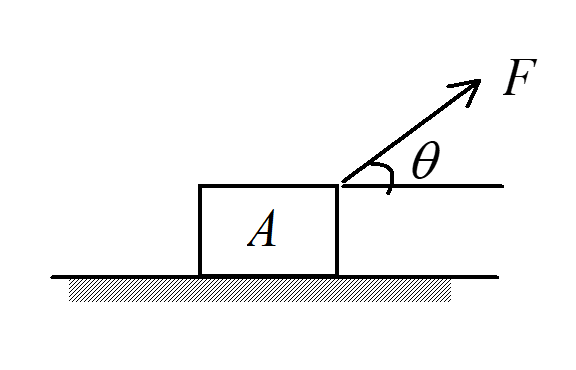
\includegraphics[width=0.15\textheight]{fig18}
            \caption{如图}\label{fig:18}
    \end{figure}
    \item 一质点从静止出发沿半径$R=1m$的圆周运动,其角加速度随时间$t$的变化规律是 (SI), 求质点从出发到$t$时刻走过的路程$S$.
        
\end{enumerate}

\section{习题参考答案}
\subsection*{一、填空题}
\begin{enumerate}
    \item 升降机内地板上放有物体$A$, 其上再放另一物体$B$, 二者的质量分别为$M_A$、$M_B$.当升降机以加速度$a$向下加速运动时$(a<g)$, 物体$A$对升降机地板的压力大小$N=\anl{$(M_A+M_B)(g-a)$}$.  
    \item 如图所示 \ref{Fig:12} , 一个小物体$A$靠在一辆小车的竖直前壁上,$A$和车壁间静摩擦系数是$\mu_s$,若要使物体$A$不致掉下来,小车的加速度的最小值应为$a=\anl{$g/ \mu _s$}$.
    \begin{figure}[H]
        \centering
        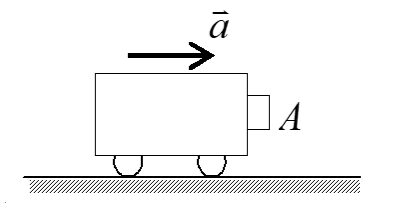
\includegraphics[width=0.15\textheight]{fig12}
            \caption{如图}\label{Fig:12}
    \end{figure}
    \item 如图 \ref{Fig:13} , 一圆锥摆摆长为$l$、摆锤质量为$m$,在水平面上作匀速圆周运动,摆线与铅直线夹角$\theta$,则摆线的张力$T=\anl{$\frac{mg}{\mathrm{cos}\theta}$}$.摆锤的速率$v=\anl{$\sqrt{\frac{gl\mathrm{sin}^2\theta}{\mathrm{cos}\theta}}$}$.
    \begin{figure}[H]
        \centering
        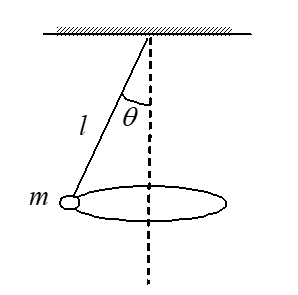
\includegraphics[width=0.15\textheight]{fig13}
            \caption{如图}\label{Fig:13}
    \end{figure}
\end{enumerate}
\subsection*{二、选择题}
\begin{enumerate}
    \item  如图 \ref{Fig:14} , 一只质量为$m$的猴,原来抓住一根用绳吊在天花板上的质量为$M$的直杆,悬线突然断开,小猴则沿杆子竖直向上爬以保持它离地面的高度不变,此时直杆下落的加速度为( D )
    \fourch{$g$ ;}{$\frac{m}{M}g$ ;}{$\frac{M+m}{M-m}g$ ;}{$\frac{M+m}{M}G$ .}
    \begin{figure}[H]
        \centering
        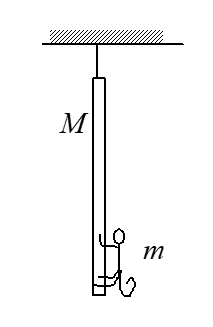
\includegraphics[width=0.06\textheight]{fig14}
            \caption{如图}\label{Fig:14}
    \end{figure}

    \begin{note}
        \textcolor{red}{先受力分析, 再计算}
        \begin{figure}[H]
            \begin{minipage}[ht]{0.6\linewidth}
                \begin{table}[H]
                    \begin{tabular}{l}
                       \qquad 计算过程:\\
                       \qquad \qquad $F=mg$ \\
                        \qquad \qquad   $F+Mg = Ma$ \\
                        \qquad \qquad $a = \frac{M+m}{M}g$\\ 
                    \end{tabular}
                \end{table}  
            \end{minipage}
            \begin{minipage}[H]{0.3\linewidth}
                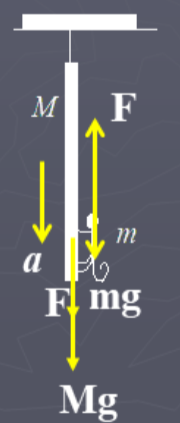
\includegraphics[width=0.06\textheight]{ans8}
            \end{minipage}
        \end{figure}
    \end{note}
    \item 一段路面水平的公路,转弯处轨道半径为$R$,汽车轮胎与路面间的摩擦系数为$\mu$,要使汽车不致于发生侧向打滑,汽车在该处的行驶速率( B )
    \twoch{不得小于$\sqrt{\mu gR}$ ;}{不得大于$\sqrt{\mu gR}$ ;}{必须等于$\sqrt{2gR}$ ;}{还应由汽车的质量$M$决定 .}
    \begin{note}
        \textcolor{red}{对车子受力分析即可:}
        \begin{figure}[H]
            \centering
            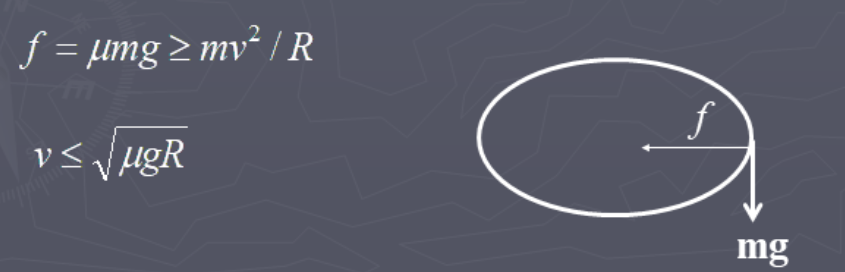
\includegraphics[width=0.30\textheight]{ans9}
        \end{figure}
    \end{note}
    \item 质量分别为$m_1$和$m_2$的两滑块$A$和$B$通过一轻弹簧水平连结后置于水平桌面上,滑块与桌面间的摩擦系数均为$\mu$, 系统在水平拉力$F$作用下匀速运动,如图所示\ref{Fig:15}。如突然撤消拉力,则刚撤消后瞬间,二者的加速度$a_A$和$a_B$分别为( D ) 
    \begin{figure}[ht]
        \begin{minipage}[ht]{0.4\linewidth}
           \begin{table}[H]
               \begin{tabular}{c}
                  \qquad   (A)\ $a_A=0, a_B=0$;\\
                  \qquad  (B)\ $a_A>0, a_B<0$;\\
                  \qquad  (C)\ $a_A<0, a_B>0$;\\
                  \qquad  (D)\ $a_A<0, a_B=0$.
               \end{tabular}
           \end{table}
        \end{minipage}
        \begin{minipage}[H]{0.5\linewidth}
            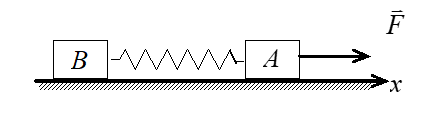
\includegraphics[width=0.25\textheight]{fig15}
            \caption{如图}\label{Fig:15}
        \end{minipage}
    \end{figure}
    \begin{note}
        \textcolor{red}{对物体受力分析: }
        \begin{figure}[H]
            \centering
            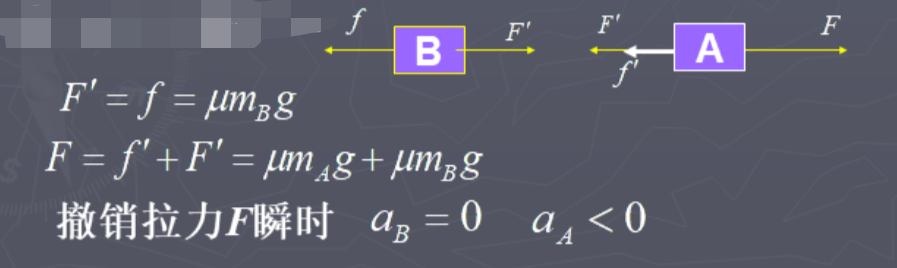
\includegraphics[width=0.30\textheight]{ans10}
        \end{figure}
    \end{note}
\end{enumerate}
\subsection*{三、计算题}
\begin{enumerate}
    \item 质量为$m$的质点沿$x$轴正向运动: 设质点通过坐标点为$x$时的速度为$v=kx$($k$为常数), 求作用在质点的合外力及质点从$x=x_0$到$x=2x_0$处所需的时间$t$.
    \begin{solution}
        $v = kx$, 加速度 $a = \frac{\mathrm{d}v}{\mathrm{d}t}=\frac{k\mathrm{d}x}{\mathrm{d}t}=kv=k^2x$\\
        $\therefore F = ma = mk^2x $\ \ $\therefore v = kx \Longrightarrow \frac{\mathrm{d}x}{\mathrm{d}t}=kx$\\ 
        $\therefore \displaystyle{\int_{x_0}^{2x_0}\frac{\mathrm{d}x}{x}=\int_0^t k\mathrm{d}t}$ \  $\therefore t = \frac{\mathrm{ln2}}{k}$.
    \end{solution}
    \item 如图 \ref{Fig:16}, 在光滑水平桌面上,有两个物体$A$和$B$紧靠在一起.它们的质量分别为$m_A=2kg$, $m_B=1kg$. 今用一水平力$F=3N$推物体$B$,求$B$推$A$的力$f$. 
    \begin{figure}[H]
        \centering
        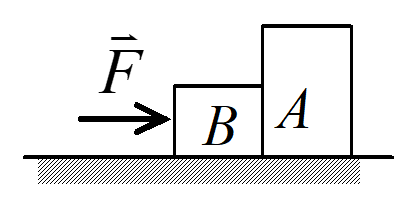
\includegraphics[width=0.15\textheight]{fig16}
            \caption{如图}\label{Fig:16}
    \end{figure}
    \begin{solution}
        看图: 
        \begin{figure}[H]
            \centering
            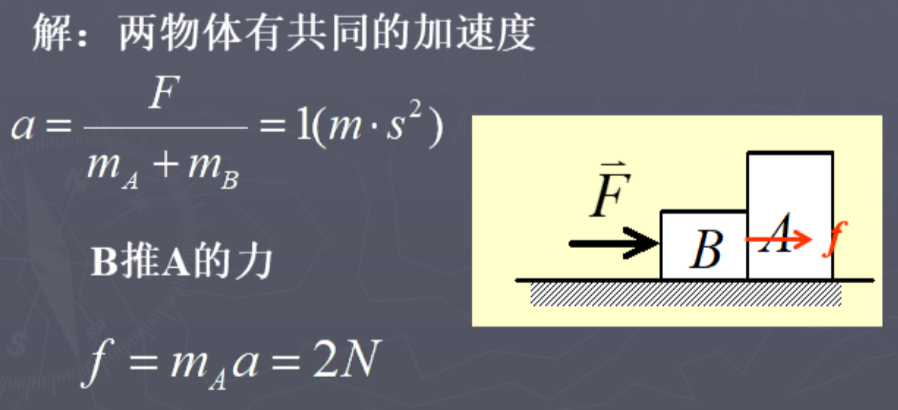
\includegraphics[width=0.38\textheight]{ans12}
        \end{figure}
    \end{solution}
    \item 如图所示 \ref{Fig:17}, 质量为$m$的物体用细绳水平拉住,静止在倾角为$\theta$的固定的光滑斜面上,求斜面给物体的支持力.
    \begin{figure}[H]
        \centering
        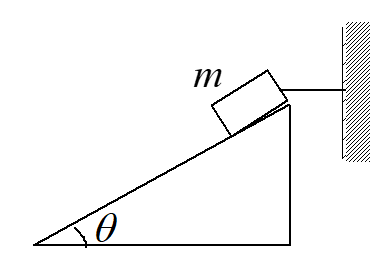
\includegraphics[width=0.15\textheight]{fig17}
            \caption{如图}\label{Fig:17}
    \end{figure}
    \begin{solution}
        看图: 
        \begin{figure}[H]
            \centering
            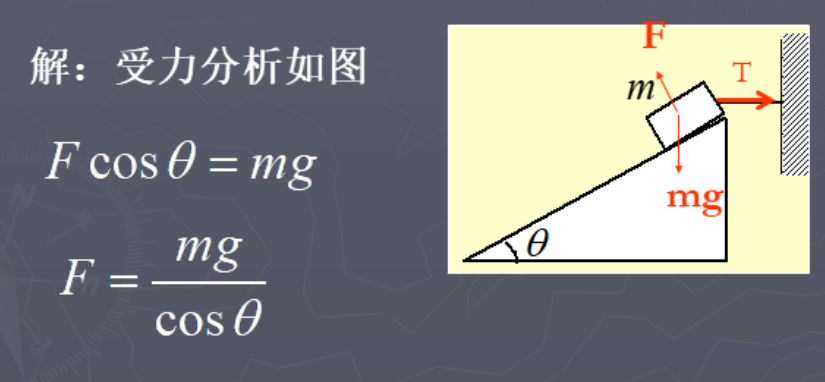
\includegraphics[width=0.25\textheight]{ans11}
        \end{figure}
    \end{solution}

     \item 如图 \ref{Fig:18} ,水平地面上放一物体$A$, 它与地面间的滑动摩擦系数为$\mu$.现加一恒力$\vec{F}$如图所示. 欲使物体$A$有最大加速度,求恒力$\vec{F}$与水平方向夹角$\theta$.
     \begin{figure}[H]
        \centering
        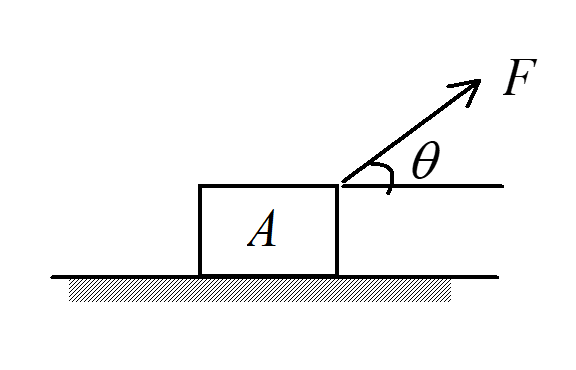
\includegraphics[width=0.15\textheight]{fig18}
            \caption{如图}\label{Fig:18}
    \end{figure}
    \begin{solution}
        看图: 
        \begin{figure}[H]
            \centering
            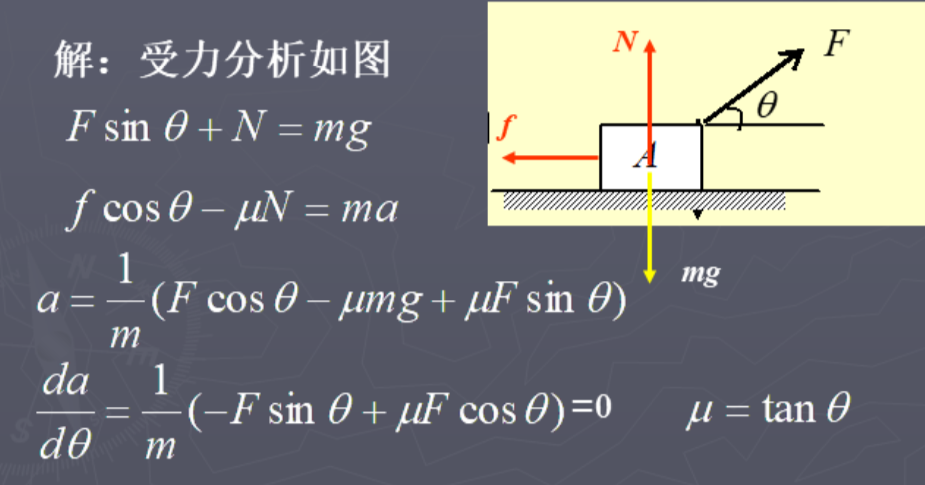
\includegraphics[width=0.38\textheight]{ans13}
        \end{figure}
    \end{solution}
    \item 一质点从静止出发沿半径$R=1m$的圆周运动,其角加速度随时间$t$的变化规律是 $\beta = 12t^2-6t$ (SI), 求质点从出发到$t$时刻走过的路程$S$.
    \begin{solution}

        \begin{figure}[ht]
            \begin{minipage}[ht]{0.7\linewidth}
                \begin{table}[H]
                    \begin{tabular}{l}
                       \qquad $\beta = \frac{\mathrm{d}\omega}{\mathrm{d}t}\Longrightarrow \mathrm{d}w=\beta \mathrm{d}t$, $\displaystyle{\int_0^\omega \mathrm{d}w = \int_0^t(12t^2-6t)\mathrm{d}t}$\\
                        
                       \qquad 角速度 $w = 4t^3-3t^2$, 令$\omega = 0$, 得$t_1=\frac{3}{4}s$. \\
                       \qquad 又$\because \omega = \frac{\mathrm{d}\theta}{\mathrm{d}t}$\ \ $\displaystyle{\int_0^{\theta}\mathrm{d}\theta = \displaystyle{\int_0^t(4t^3-3t^2)\mathrm{d}t}}$, 
                $\theta = t^4-t^3$
                    \end{tabular}
                \end{table}
            \end{minipage}
            \begin{minipage}[H]{0.25\linewidth}
                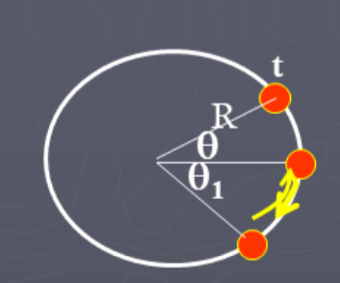
\includegraphics[width=0.13\textheight]{ans14}
            \end{minipage}
        \end{figure}
        \begin{enumerate}
            \item[1)] 当$t<(3/4)s$时\\
            质点角坐标为负(顺时针转)对应路程: $S=|R\theta|=(t^3-t^4) m$
            \item[2)] 当$t>(3/4)s$时\\
            质点开始逆时针转, 路程由开始两部分组成 $S=R(\theta-\theta_1)+R|\theta_1|= (t^4-t^3+0.2) m$
        \end{enumerate}
    \end{solution}    
\end{enumerate}